\documentclass[conference]{IEEEtran}
\IEEEoverridecommandlockouts
% The preceding line is only needed to identify funding in the first footnote. If that is unneeded, please comment it out.
\usepackage{cite}
\usepackage{amsmath,amssymb,amsfonts}
\usepackage{algorithmic}
\usepackage{graphicx}
\usepackage{textcomp}
\usepackage{xcolor}
\usepackage{tabularx}
\usepackage{multirow}
\usepackage{graphics} % for pdf, bitmapped graphics files
\usepackage{subfig}
\usepackage{subcaption}
\usepackage{hyperref}
\usepackage{academicons}
\usepackage{xcolor}
\usepackage{listings}
\def\BibTeX{{\rm B\kern-.05em{\sc i\kern-.025em b}\kern-.08em
		T\kern-.1667em\lower.7ex\hbox{E}\kern-.125emX}}
% Gráficas en MATLAB
\usepackage{tikz, pgfplots}
% Color Enlace
\definecolor{colorEnlace}{RGB}{0, 0, 0}
\hypersetup{
	colorlinks=true,
	linkcolor=colorEnlace,
	citecolor=colorEnlace,
	urlcolor=colorEnlace,
	pdfauthor={Davis Bremdow Salazar Roa},
	pdftitle={Diseño de controlador PID}
}
% Control 
\usepackage{amsmath}
\begin{document}
	
	\title{Experiencia N°4 - Diseño de Controlador PID}
	% Ing. Diego Darcy Arredondo Huarac
	\author{	
		\IEEEauthorblockN{Davis Bremdow Salazar Roa}
		\IEEEauthorblockA{Universidad Nacional de San Antonio Abad del Cusco}
		\textit{Escuela Profesional de Ingeniería Electrónica}\\
		\textit{Laboratorio de Control I}\\
		200353 \\\\
		Cusco, Perú
	}
	
	\maketitle
	
	\begin{abstract}
		The document outlines the design of a PID controller using the Ziegler-Nichols tuning method for an analog control system. The objectives include designing controllers for underdamped and overdamped cases, aiming to reduce overshoot and response time. For the underdamped case, calculations for parameters \( k_p \), \( k_i \), and \( k_d \) are based on a derived transfer function, with the system tuned to cut overshoot by half. For the overdamped case, similar calculations optimize response time. Simulations in MATLAB/Simulink demonstrate step and impulse responses, highlighting improvements in control. Additionally, the document presents PID circuit designs with specified resistor and capacitor values for each damping case, along with simulated output graphs for analysis.
	\end{abstract}
	
	\begin{IEEEkeywords}
		PID controller design, response optimization, Ziegler-Nichols method, analog control system, underdamped response, overdamped response, transfer function, gain tuning, MATLAB/Simulink simulation, circuit design, 
	\end{IEEEkeywords}
	
	\section{Introducción}
	En esta experiencia de laboratorio se explora la implementación de un controlador PID para ajustar la respuesta de sistemas de segundo orden, tanto subamortiguados como sobreamortiguados. El objetivo principal es modificar la salida de estos sistemas para alcanzar un comportamiento deseado, a pesar de las perturbaciones externas.
	
	El controlador PID (Proporcional, Integral, Derivativo) actúa sobre la diferencia entre el valor deseado y el actual de la variable de salida, conocido como error. Mediante el uso de la técnica de Ziegler-Nichols, se diseñan y simulan controladores PID que buscan optimizar parámetros como el sobrepico y el tiempo de respuesta, mejorando así la estabilidad y eficiencia del sistema.
	
	El documento detalla los procedimientos para calcular los coeficientes del controlador PID, utilizando simulaciones para validar los resultados. Se presentan casos específicos para sistemas subamortiguados y sobreamortiguados, demostrando cómo un controlador PID bien ajustado puede mejorar significativamente la performance del sistema.
	
	\section{Objetivos}
	
	\begin{itemize}
		\item Diseñar un controlador PID para reducir el sobreimpulso y tiempo de establecimiento
		\item Implementación de un controlador PID mediante Amp. Operacionales
	\end{itemize}
	
	\section{Diseño de un controlador PID analógico mediante la técnica de Ziegler - Nichols}
	El control PID (Proporcional Integral y Derivativo) también conocido como el método de sintonización es una forma de modificar el comportamiento de un sistema mediante la adición de 3 elementos (un proporcional, un integrador y  derivador) con los cuales al realizar un ajuste a sus parámetros, se pueden modificar el comportamiento de un sistema.
	
	Para la sintonización de los parámetros $k_p, k_i, k_d$ es necesario aplicar ciertas reglas ya establecidas que nos permitirán tener un punto de partida ideal para aproximar el comportamiento del sistema a lo deseado según el planteamiento del sistema, de forma general un control PID se describe matemáticamente en \ref{eq:mat-pid} y del podremos destacar 3 constantes para su sintonización, entre ellas, se tiene: \\
	
	$K_p$ : Constante proporcional \\
	$K_i = \frac{K_p}{T_i}$ : Constante integral \\
	$K_d = K_pT_d$ : Constante derivativa \\
	
	\begin{equation}
		K_p(1 + \frac{1}{T_iS} + T_dS)
		\label{eq:mat-pid}
	\end{equation}
	
	Dentro de los casos o métodos que se pueden aplicar para la sintonización de parámetros mediante la técnica de Zigler - Nichols, se tienen 2 formas las cuales dependen de la respuesta del sistema frente a una entrada escalón unitario.
	
	\subsection{\textbf{Caso subamortiguado reducir el sobre impulso a la mitad}}
	
	Para el caso del sistema subamortiguado, fue necesario aplicar el segundo método debido al sobreimpulso en su respuesta frente al escalón unitario, para este método se debe variar con la constante proporcional $K_p$ haciendo que el resto de parámetros sea cero, hasta que la salida del sistema oscile, considerando el sistema de 2do orden mostrado en la figura \ref{fig:planta-sistema}.
	
	\begin{figure}[h]
		\centering
		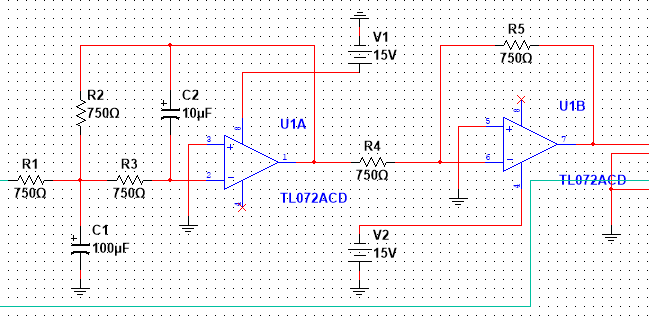
\includegraphics[width=0.4\textwidth]{media1/planta-sistema}
		\caption{Sistema de segundo orden}
		\label{fig:planta-sistema}
	\end{figure}
	
	Se puede establecer que la función de transferencia aproximada, según los polos de trabajo asignados, serán:
	
	\begin{equation}
		H(s) = \frac{65}{s^2 + 2s + 65}
		\label{eq:ft-planta}
	\end{equation}
	
	Sin embargo analizando este sistema mediante el lugar geométrico de las raíces, se puede notar que este sistema no oscilara para ningún valor de $K_p$ debido a que ramas no se interceptan con el eje imaginario para ningún valor de ganancia, tal y como se puede apreciar en la figura \ref{fig:lgr-planta}
	
	\begin{figure}[h]
		\centering
		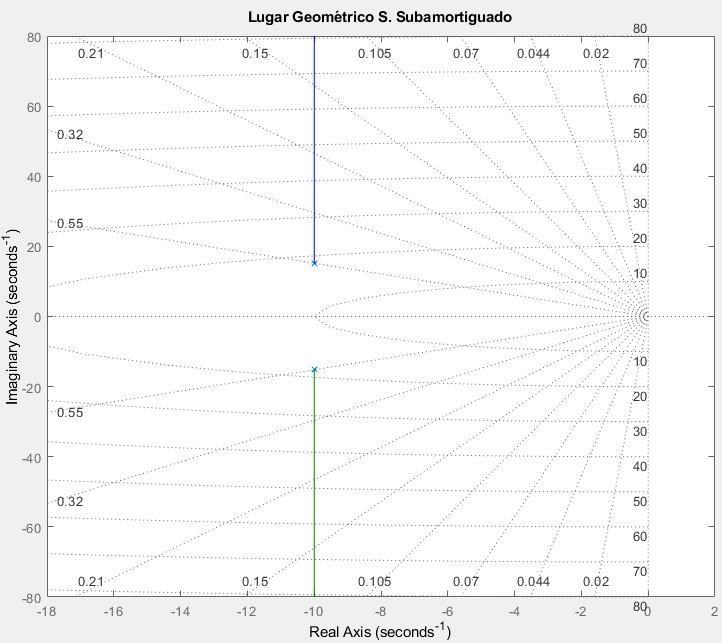
\includegraphics[width=0.4\textwidth]{media/lgr-planta}
		\caption{Lugar geométrico de las raíces del sistema}
		\label{fig:lgr-planta}
	\end{figure}
	
	Por lo tanto no será posible aplicar ningún método según Ziegler-Nichos por lo que será necesario agregar un integrados un polo en el origen para que el sistema se vuelva inestable (oscile) para un determinado valor de ganancia, ahora conocida como $K_c$ o ganancia crítica.
	
	Por lo tanto la nueva función de transferencia se describe en \ref{eq:ft-planta-polo} y mediante este arreglo el sistema oscilara para un valor de $K_c$ que establezca raíces en el eje imaginario, para determinar este valor se puede hacer uso del criterio de estabilidad de Routh Hurtwitz en uno de sus casos especiales, la cual define que cuando todas las constantes de una de las filas del criterio sea igual a cero se tendrán raíces conjugadas en el eje imaginario.
	
	\begin{equation}
		H(s) = \frac{65K_c}{s^3 + 2s^2 + 65s}
		\label{eq:ft-planta-polo}
	\end{equation}
	
	Antes de aplicar el criterio de estabilidad será necesario aplicar retroalimentación unitaria cuya función de transferencia se define en al sistema considerando $K_c$ como la ganancia del sistema y la cual se analizará para obtener el valor que haga oscilar al sistema.
	
	\begin{equation}
		H(s) = \frac{65K_c}{s^3 + 2s^2 + 65s + 65K_c}
		\label{eq:ft-planta-retroalimentacion}
	\end{equation}
	
	Una de vez definido el polinomio denominador se aplica el criterio obteniendo la siguiente relación definida en \ref{eq:constante-critica}
	\begin{align}
		S0 : 65(2) - 65K_c &= 0 \\
		K_c &= 2
		\label{eq:constante-critica}
	\end{align}
	
	Con este valor definido se puede hacer uso de la relación $s = j\omega$ para obtener la frecuencia angular y con el ello el periodo critico $P_c$ mediante el cual se podrán calcular los parámetros $K_p, K_i, K_d$ que nos permitirán iniciar con la sintonización fina para adecuar el comportamiento del sistema reduciendo el sobreimpulso en un 50\%
	
	Reemplazando $s =j\omega$ se tiene:
	\begin{equation}
		P(j\omega) = (j\omega)^3 +2 (j\omega)^2 + 65(j\omega) + 65K_c = 0
		\label{eq:ft-jw}
	\end{equation}
	
	Como en \ref{eq:ft-jw} se tiene una expresión compleja se debe separar la parte real e imaginaria e igualarlas a cero, reduciendo la función obtenida y remplazando el valor $K_c$ se tiene las siguientes relaciones
	
	\begin{align}
		65K_c - 2\omega &= 0 \\
		\omega^2 &= \frac{65(2)}{2} \\
		\omega &= \sqrt{65} \\
		\omega &= 8.06 \\
		\label{eq:frecuencia-critica}
	\end{align}
	
	Para la obtención del periodo, se hace uso de $\omega_c = \frac{2\pi}{P_c}$, siendo el periodo critico igual $P_c = \frac{2\pi}{8.06} = 0.7793 \label{eq:periodo-critico}$.
	
	Una vez definido el periodo crítico, solo basta con definir los valores de las constantes PID en función a la tabla \ref{fig:pid-reglas-2}
	
	\begin{figure}[h]
		\centering
		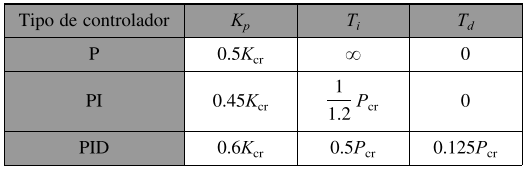
\includegraphics[width=0.4\textwidth]{media/pid-reglas-2}
		\caption{Reglas de sintonía de Ziegle Nichols en función de Kc y Pc}
		\label{fig:pid-reglas-2}
	\end{figure}
	
	Siendo así que: \\
	$K_p = 0.6*K_c$ \\
	$K_i = \frac{K_p}{T_i}$ \\
	$K_p = T_d*K_p$ \\
	
	Obteniendo así que $K_p = 1.2$, $K_i = 3.080$ y $K_d = 0.1168$ siendo estos los valores iniciales con los cuales se realizara la sintonización y se adecuaran los mismos para reducir el sobreimpulso en un 50\%, analizando y realizando las pruebas con diferentes valores para obtener la condiciones necesarias se obtuvo que los valores ideales serán $K_p = 27$, $K_i = 69.29$ y $K_d = 2.6302$ valores que se obtuvieron al multiplicar a cada constante por un factor de 22.5.
	
	La salida del sistema sin el control PID y los cambios en la respuesta del sistema mediante el uso del control PID se puede apreciar en la figura \ref{fig:pid-subamortiguado}, las cuales se definieron haciendo uso del entorno de programación visual Simulink y cuyo esquema se aprecia en la figura \ref{fig:subamortiguado-simulink}
	
	
	\begin{figure}[h]
		\centering
		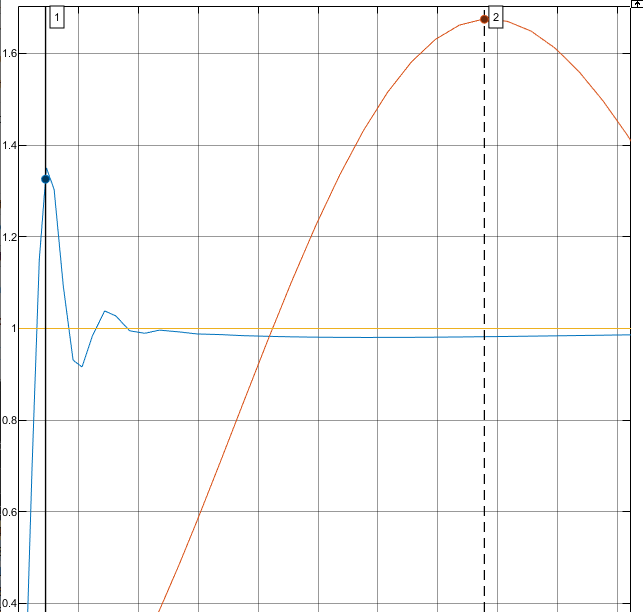
\includegraphics[width=0.4\textwidth]{media1/pid-subamortiguado}
		\caption{Controlador PID para el sistema subamortiguado}
		\label{fig:pid-subamortiguado}
	\end{figure}
	
	
	\begin{figure}[h]
		\centering
		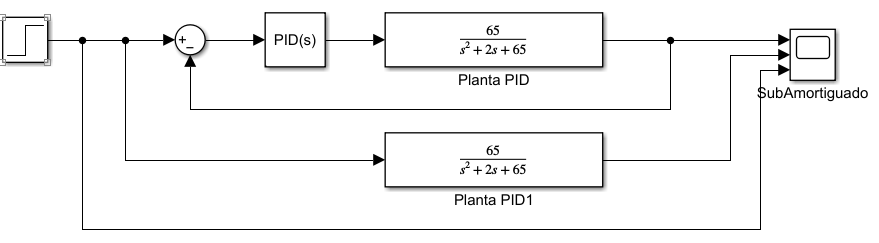
\includegraphics[width=0.5\textwidth]{media1/subamortiguado-simulink}
		\caption{Sistema subamortiguado simulink}
		\label{fig:subamortiguado-simulink}
	\end{figure}
	
	
	\subsection{\textbf{Caso sobreamortiguado reducir el tiempo de establecimiento $T_s$ a la mitad}}
	
	Para el caso del sistema sobre amortiguado lo que se busca es reducir el tiempo de establecimiento en al menos un 50\%, al analizar la respuesta del sistema de segundo orden según \cite{ogata2015} se puede apreciar que esta tiene una salida sigmoidal como se aprecia en la figura \ref{fig:respuesta-escalon-sobre}, siendo la función de transferencia del sistema definida en \ref{eq:ft-sobreamortiguado}
	
	\begin{equation}
		H(s) = \frac{215.25}{s^2 + 31s + 215.25}
		\label{eq:ft-sobreamortiguado}
	\end{equation}
	
	\begin{figure}[h]
		\centering
		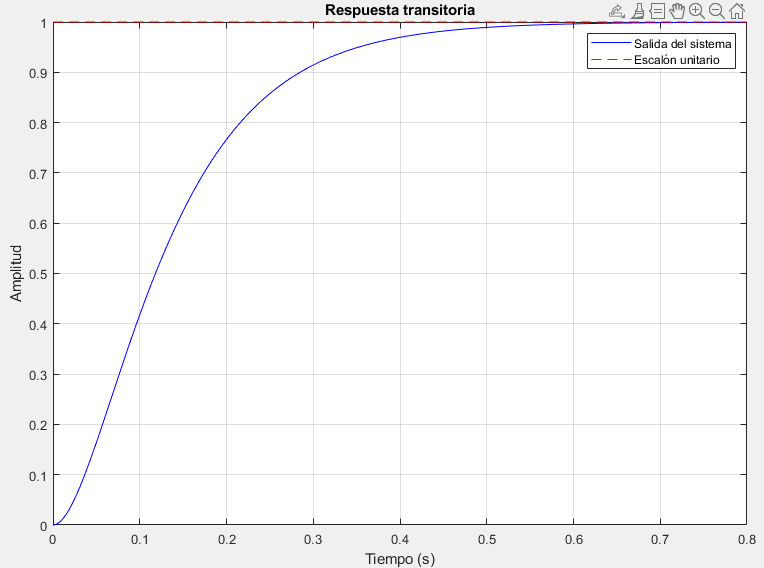
\includegraphics[width=0.4\textwidth]{media1/respuesta-escalon-sobre}
		\caption{Respuesta al escalón unitario del sistema sobreamortiguado}
		\label{fig:respuesta-escalon-sobre}
	\end{figure}
	
	La salida de este sistema, nos permite trabajar bajo el primer criterio, según Ziegler-Nichols el cual establece el calculo de los 2 constantes de tiempo $L$ y $\tau$ para definir los valores de las ganancias proporcional, integral y derivativa, esta relación se puede apreciar en la figura \ref{fig:pid-reglas-1}
	
	\begin{figure}[h]
		\centering
		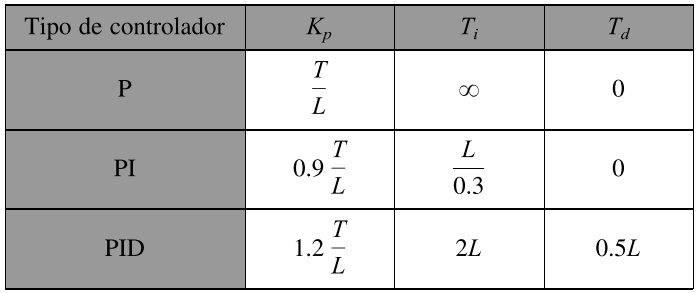
\includegraphics[width=0.4\textwidth]{media/pid-reglas-1}
		\caption{Método de Sintonización PID - constante de tiempo}
		\label{fig:pid-reglas-1}
	\end{figure}
	
	Además para el calculo de estas 2 constantes de tiempo es necesario determinar el punto de inflexión en la respuesta del sistema y determinar los puntos de corte, mediante el trazo de una recta tangente en el punto de inflexión y su corte en el valor máximo de la señal de entrada y el eje de tiempo o de las abcisas, para este procesamiento se hace uso de la herramienta MATLAB mediante el siguiente código de programación.
	
	\lstset{
		language=Matlab, % Define el lenguaje
		basicstyle=\ttfamily\small, % Tamaño de letra pequeño
		keywordstyle=\color{blue}, % Color de las palabras clave
		commentstyle=\color{green}, % Color de los comentarios
		stringstyle=\color{red}, % Color de las cadenas de texto
		numbers=left, % Muestra los números de línea a la izquierda
		numberstyle=\tiny\color{gray}, % Estilo de los números de línea
		stepnumber=1, % Muestra un número en cada línea
		breaklines=true, % Ajuste automático de línea
		frame=single, % Borde alrededor del código
		xleftmargin=0em, % Elimina el margen izquierdo
		framexleftmargin=0em % Elimina el espacio dentro del marco izquierdo
	}
	
	\begin{lstlisting}
		clc; clear all;
		
		num_sys = [215.25];
		den_sys = [1 31 215.25];
		
		system = tf(num_sys, den_sys);
		
		[response, t] = step(system);
		
		dy_dt = gradient(response, t);
		
		[~, max_slope_idx] = max(dy_dt);
		t_tangent = t(max_slope_idx);
		y_tangent = response(max_slope_idx);
		slope = dy_dt(max_slope_idx);
		
		t_line = linspace(t(1), t(end), 500);
		y_line = slope * (t_line - t_tangent) + y_tangent;
		
		figure;
		plot(t, response, 'b', 'Nombre a mostrar', 'Respuesta al escalon');
		hold on;
		plot(t_line, y_line, 'r--', 'Nombre a mostrar', 'Linea tangente');
		plot(t_tangent, y_tangent, 'ro', 'Nombre a mostrar', 'Punto de tangencia');
		title('Respuesta al escalon del sistema de segundo orden con linea tangente');
		xlabel('Tiempo (s)');
		ylabel('Respuesta');
		ylim([0 1.2]); % Limitar el eje y hasta 1.2
		legend;
		grid on;
		
		fprintf('Punto de tangencia: (%.4f, %.4f)\n', t_tangent, y_tangent);
		fprintf('Pendiente de la tangente: %.4f\n', slope);
	\end{lstlisting}
	
	Obteniendo mediante esto, la siguiente figura con las parámetros necesarios para el calculo de las constantes de tiempo y la cual se detallan en la figura \ref{fig:sobreamortiguado-tangente}, de la gráfica se destaca que el valor de $L=0.0194$ y de $\tau = 0.1928$.
	
	
	
	\begin{figure}[h]
		\centering
		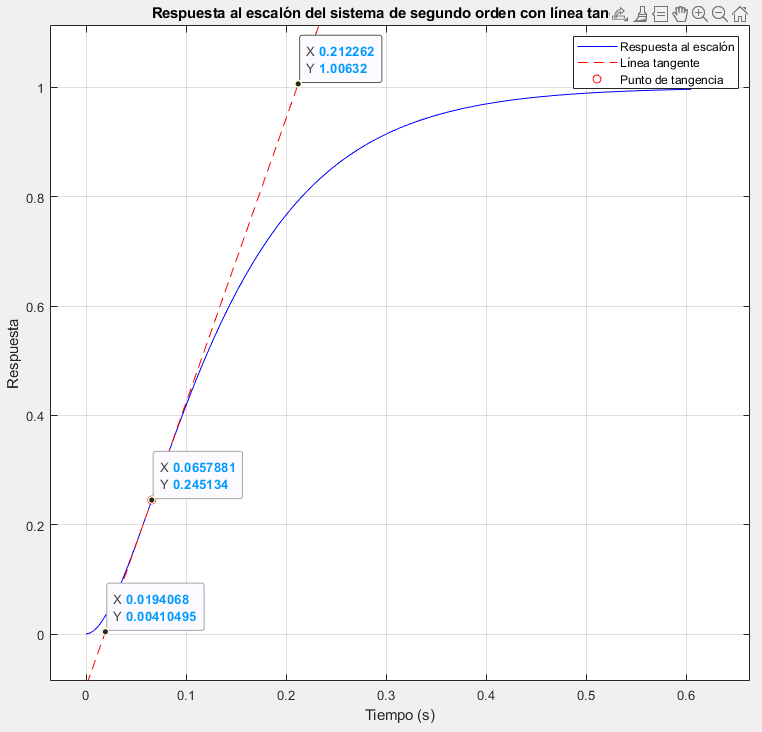
\includegraphics[width=0.4\textwidth]{media1/sobreamortiguado-tangente}
		\caption{Recta tangente en el punto de inflexión para el sistema sobreamortiguado}
		\label{fig:sobreamortiguado-tangente}
	\end{figure}
	
	Una vez con estos valores calculados, solo será necesario aplicar las relaciones definidas en la figura \ref{fig:pid-reglas-1} obtenido los valores de sintonización iniciales los cuales son:
	
	\begin{align}
		K_p &= 11.925 \\
		K_i &= 307.365 \\
		K_d &= 0.1156
	\end{align}
	
	Sin embargo estos valores a pesar de sus idealidad no son los exactos para reducir el tiempo de establecimiento a la mitad, por ello es necesario realizar un reajuste al multiplicar estas constantes por un factor de 2 obteniendo un valor de $K_p = 23.851$, $K_i = 614.7305$ y finalmente un valor de $K_d = 0.2313$
	
	Finalmente la salida del sistema aplicando control PID se muestra en la figura \ref{fig:sobreamortiguado-pid} y en el cual se puede apreciar que el tiempo de establecimiento al 2\% tiene una reducción del 60.87\% al tiempo de establecimiento original y equivalente a 0.57s, logrando reducirlo a un 0.2217s.
	
	\begin{figure}[h]
		\centering
		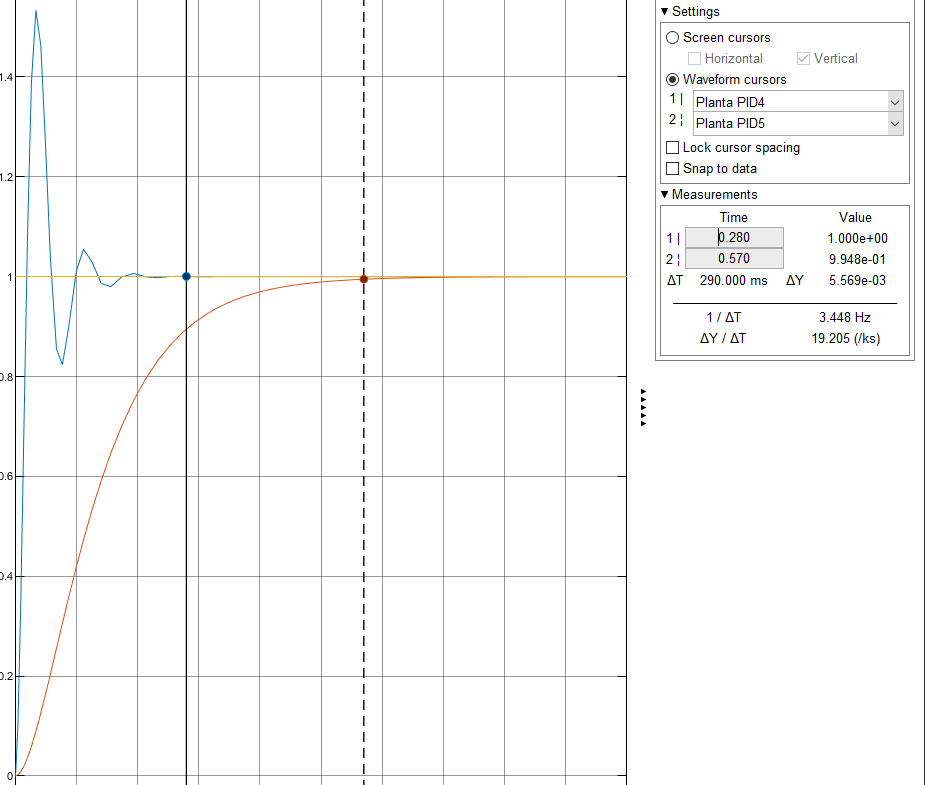
\includegraphics[width=0.4\textwidth]{media1/sobreamortiguado-pid}
		\caption{Salida del sistema luego de aplicar control PID}
		\label{fig:sobreamortiguado-pid}
	\end{figure}
	
	
	\section{simule el sistema de control en lazo cerrado mediante el software MATLAB o Simulink}
	
	Existen diferentes formas de poder simular circuitos electrónicos en MATLAB. Una de las principales es Simulink, una plataforma gráfica que permite construir modelos de sistemas dinámicos, incluyendo circuitos eléctricos mediante bloques predefinidos en las bibliotecas de Simscape Electrical y el cual fue utilizado para analizar la respuesta del sistema a las diferentes entradas propuestas.
	
	
	\subsection{\textbf{Función escalón unitario}}
	Para el caso el sistema \textbf{subamortiguado} la respuesta del sistema frente al escalón unitario se muestra en la figura \ref{fig:res-subamortguado-escalon}
	
	\begin{figure}[h]
		\centering
		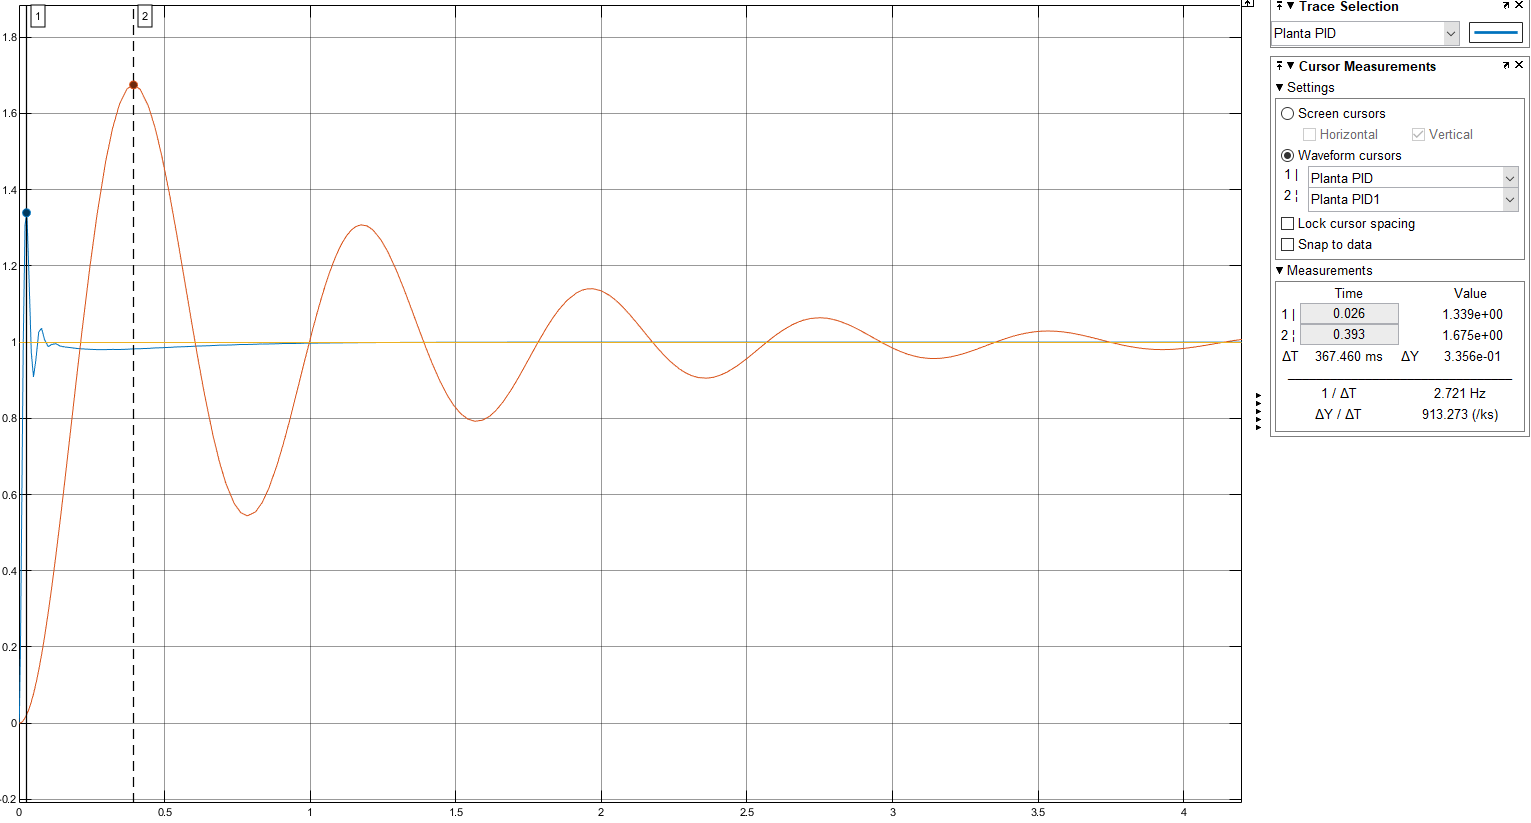
\includegraphics[width=0.35\textwidth]{media1/res-subamortguado-escalon}
		\caption{Respuesta del sistema subamortiguado frente al escalón unitario}
		\label{fig:res-subamortguado-escalon}
	\end{figure}
	
	Para el caso del sistema \textbf{sobreamortiguado} su respuesta frente al escalón unitario se muestra en la figura \ref{fig:res-sobreamortguado-escalon}
	
	
	\begin{figure}[h]
		\centering
		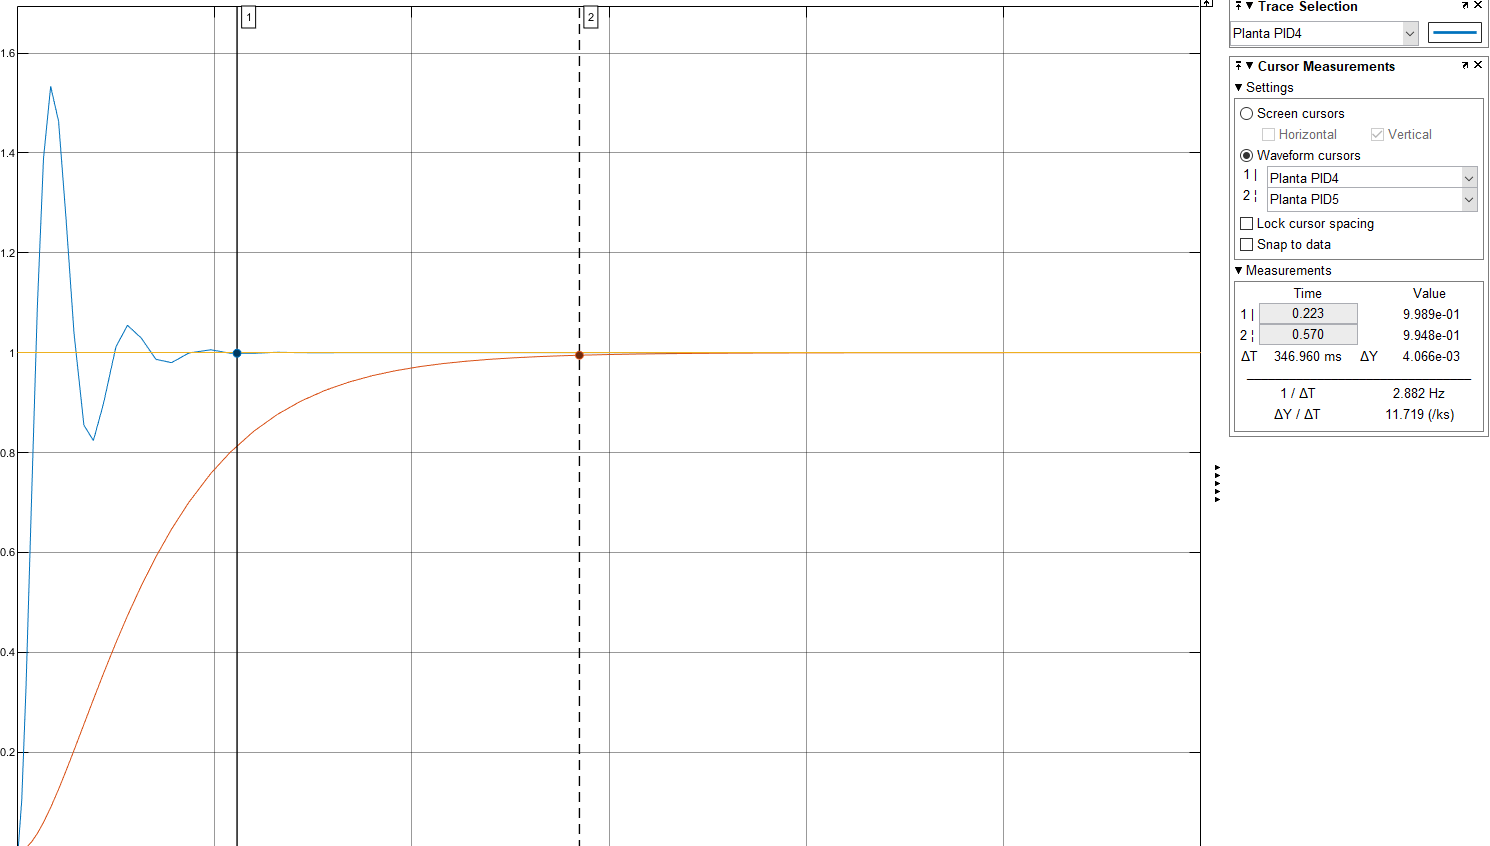
\includegraphics[width=0.4\textwidth]{media1/res-sobreamortiguado-escalon}
		\caption{Respuesta del sistema PID al escalón unitario}
		\label{fig:res-sobreamortguado-escalon}
	\end{figure}	
	
	
	\subsection{\textbf{Función impulso}}
	
	De igual forma que en los puntos previos la salida del sistema para el sistema \textbf{subamortiguado} se aprecia en la figura \ref{fig:res-subamortguado-impulso}
	
	
	\begin{figure}[h]
		\centering
		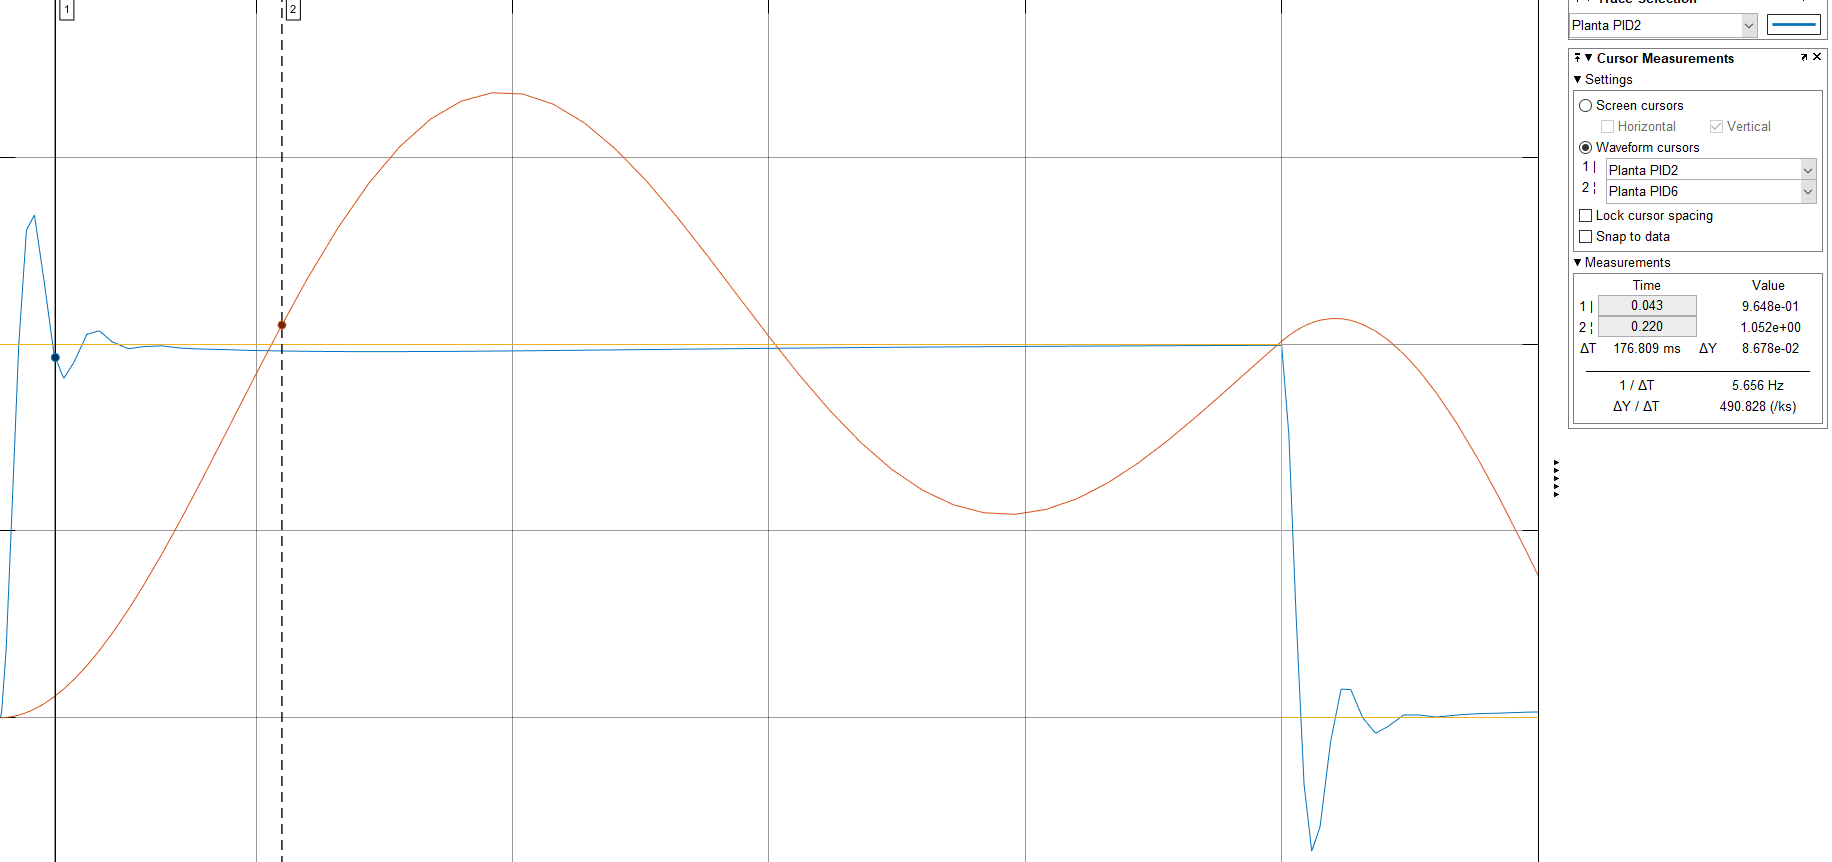
\includegraphics[width=0.4\textwidth]{media1/res-subamortguado-impulso}
		\caption{Respuesta del sistema PID frente al impulso}
		\label{fig:res-subamortguado-impulso}
	\end{figure}
	
	En el caso del sistema \textbf{sobreamortiguado} su comportamiento/salida del sistema frente al impulso, se puede apreciar en la figura \ref{fig:res-sobreamortguado-impulso}
	
	
	\begin{figure}[h]
		\centering
		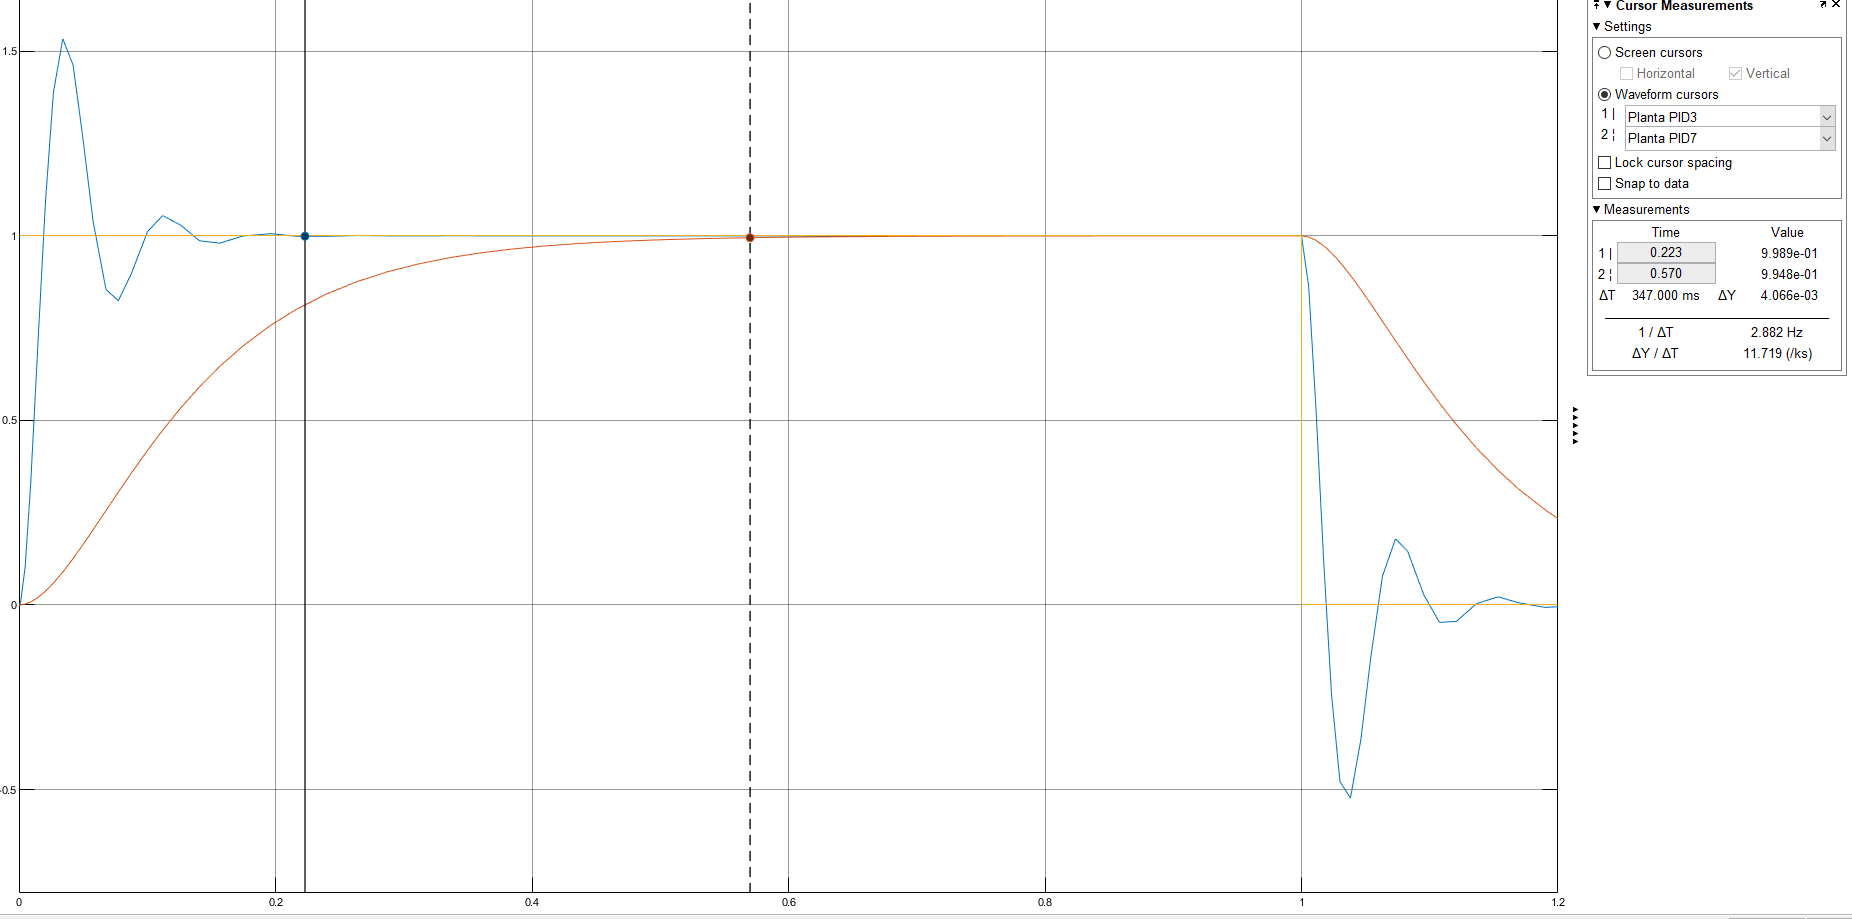
\includegraphics[width=0.4\textwidth]{media1/res-sobreamortguado-impulso}
		\caption{Respuesta del sistema de Control PID frente al impulso}
		\label{fig:res-sobreamortguado-impulso}
	\end{figure}
	
	
	\section{Descripción de las gráficas para cada caso}
	
	\subsection{Respuesta del sistema de Control PID frente al escalón unitario}
	La gráfica presenta una respuesta transiente con una subida inicial, seguida de una oscilación amortiguada hasta llegar al valor de estado estacionario.
	
	Este comportamiento refleja la capacidad del sistema de control PID para responder a cambios escalón en la entrada, ajustando la salida de manera adecuada para mantener la estabilidad y el seguimiento de la referencia.
	
	\subsection{Respuesta del sistema PID frente al impulso unitario}
	
	La gráfica muestra una respuesta transitoria con un pico inicial y luego una rápida estabilización hacia cero.
	Este comportamiento es típico de un sistema de control PID, donde la acción de control reacciona a los cambios bruscos de la entrada (impulso) para mantener la estabilidad del sistema.
	
	\section{Diseño del circuito con resistencias y capacitores para el caso Subamortiguado y sobreamortiguado}
	
	\subsection{Caso SubAmortiguado}
	
	Finalmente para el modelado del sistema de forma física mediante el uso de Amplificadores Operacionales, resistencias y capacitancias fue necesario trabajar con las constante de proporcionalidad, integral y derivativa para cada caso, eligiendo en función a los cálculos los valores comerciales más aproximados para cada elemento pasivo.
	
	Además para el desarrollo se tuvieron ciertas consideraciones para las resistencias de entrada y salida del circuito para control PID, entre ellas las resistencias $R_1 = R_2 = R_3 = R_4 = 1k[\Omega]$ para obtener una configuración de restador en el Amplificador operacional $U_1$ y las resistencias $R_7 = R_9 = R_11 = 1k [\Omega]$ para que la ganancia de parte de los controles proporcional, integral y derivativo, no se vean afectados, sin embargo para ajustar el modelamiento y obtener valores de capacitivos y de resistencia cercanos a los comerciales se tuvo en cuenta un factor en $R_12 = 4.7K [\Omega]$ para facilitar el diseño en ambos circuitos.
	
	Para el resto de elemento de igual forma se definieron los siguientes valores estableciendo las capacitancias como valores constantes debido a la dificultad y poca disponibilidad comercial de estos elementos, teniendo así que $C_1 = 22uF$ y $C_2 = 100uF$ y las resistencias $R_5 = 750\Omega$, $R_6 = 4.7k\Omega$, $R_8 = 2.7k\Omega$, y finalmente $R_10 = 1.2k\Omega$, siendo el circuito simulado en NI Multisim, el se muestra en la figura \ref{fig:circuito-subamortiguado}
	
	Otro apartado a destacar es el sistema de control PID para el caso subamortiguado y cuyo comportamiento matemático se describió de la siguiente forma, mediante la ecuación \ref{eq:control-pid-subamortiguado}
	
	\begin{align}
		G(s) &= K_p +  \frac{K_i}{s} + Kds \\
		G(s) &= 30 +  \frac{76.988}{s} + 0.55s
		\label{eq:control-pid-subamortiguado}
	\end{align}
	
	\begin{figure}[h]
		\centering
		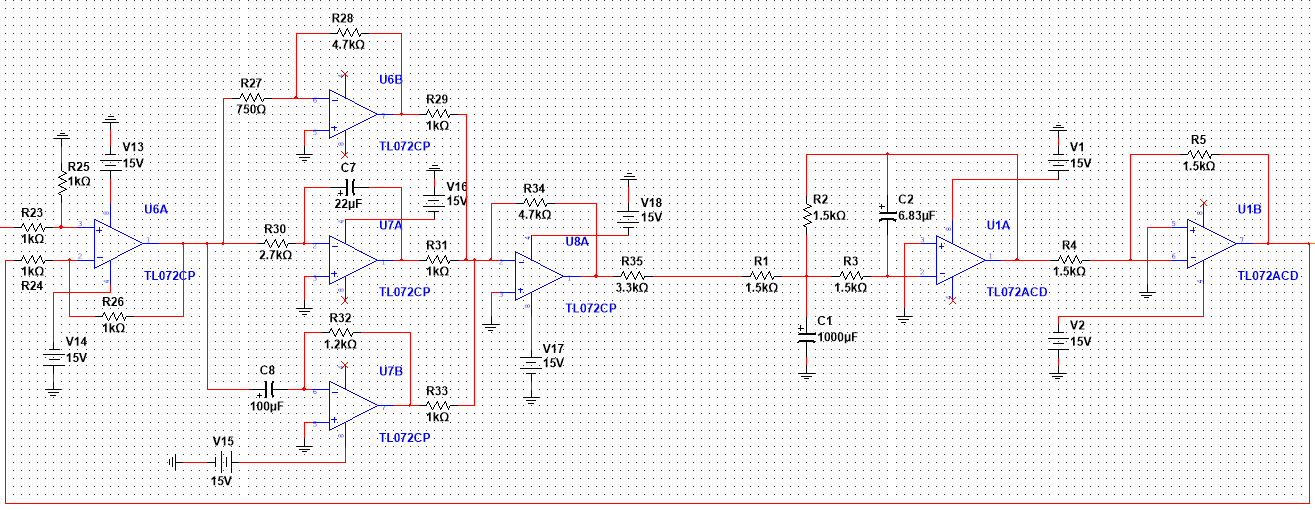
\includegraphics[width=0.5\textwidth]{media1/circuito-subamortiguado}
		\caption{Circuito diseñado para el sistema subamortiguado}
		\label{fig:circuito-subamortiguado}
	\end{figure}
	
	La respuesta del sistema modificado mediante el control PID se puede apreciar en la figura \ref{fig:respuesta-circuito-sub} y en a cual se puede apreciar la reducción del sobreimpulso a menos de la mitad, además de apreciarse ciertas variaciones en el tiempo de establecimiento debido a que no se trabajo la simulación con los valores exactos para los elementos debido a que estos valores calculados no existen comercialmente.
	
	\begin{figure}[h]
		\centering
		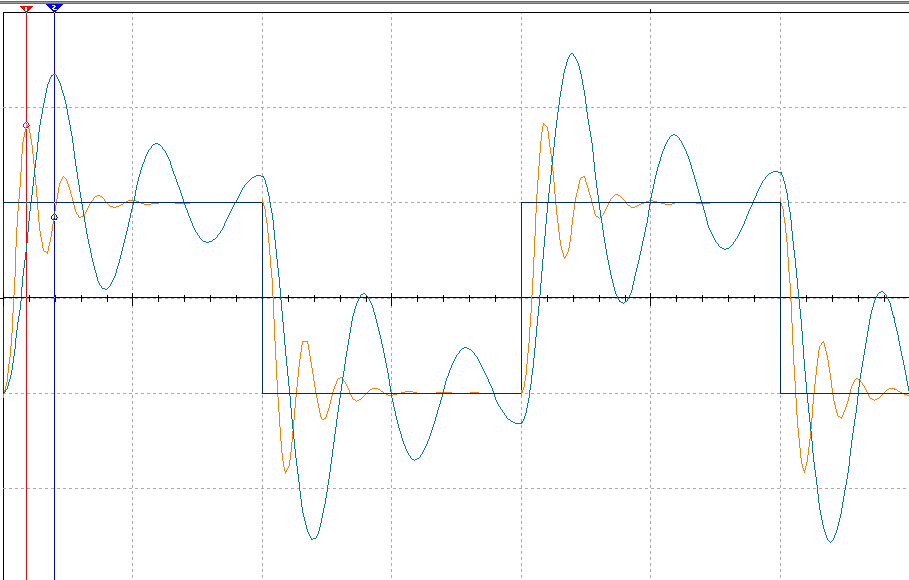
\includegraphics[width=0.5\textwidth]{media1/respuesta-circuito-sub}
		\caption{Respuesta del sistema frente a una señal cuadrada}
		\label{fig:respuesta-circuito-sub}
	\end{figure}
	
	\subsection{Caso SobreAmortiguado}
	
	Para el caso del sistema sobreamortiguado también se consideraron las condiciones circuitales propuestas para el circuito subamortiguado alterando para este segundo caso las ganancias proporcional, integral y derivativa para cada elemento pasivo, siendo que para  $C_1 = 22uF$ y $C_2 = 47uF$ y las resistencias $R_5 = 220\Omega$, $R_6 = 1.5k\Omega$, $R_8 = 330k\Omega$ y finalmente $R_10 = 1k\Omega$
	
	En el caso del sistema sobreamortiguado el sistema de control esta caracterizado mediante la siguiente expresión matemática definida en \ref{eq:control-pid-sobreamortiguado}
	\begin{align}
		G(s) &= K_p +  \frac{K_i}{s} + Kds \\
		G(s) &= 35.77 +  \frac{614.7305}{s} + 0.2313s
		\label{eq:control-pid-sobreamortiguado}
	\end{align}
	
	El circuito final para el sistema sobreamortiguado se aprecia en la figura \ref{fig:circuito-sobreamortiguado}
	
	\begin{figure}[h]
		\centering
		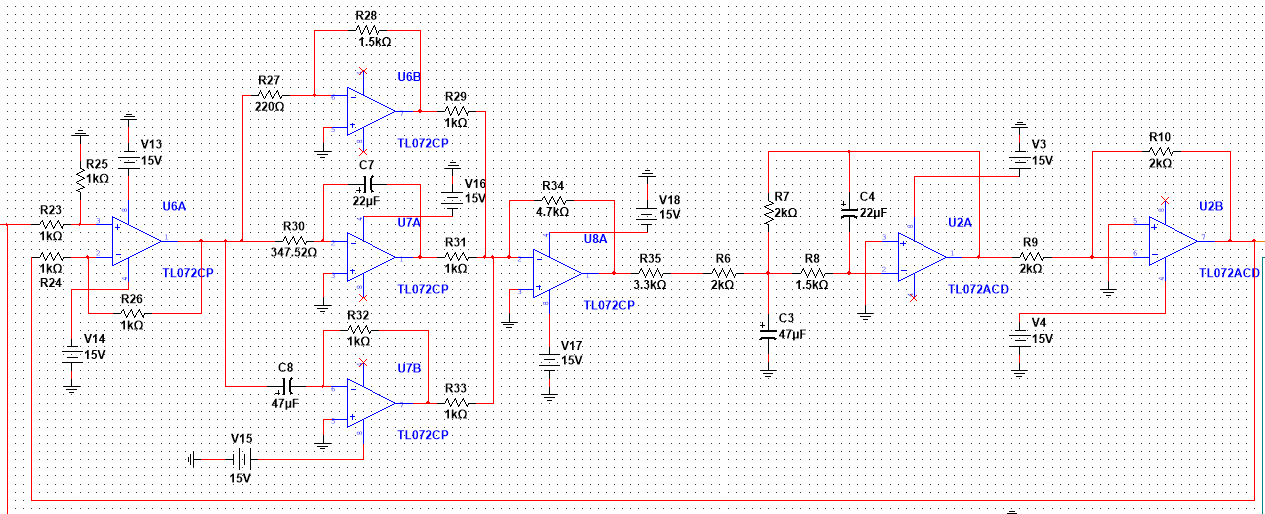
\includegraphics[width=0.5\textwidth]{media1/circuito-sobreamortiguado}
		\caption{Circuito diseñado para el sistema sobreamortiguado PID}
		\label{fig:circuito-sobreamortiguado}
	\end{figure}
	
	Y la salida del sistema frente una señal de impulsos cuadrados, se muestra en la figura \ref{fig:respuesta-circuito-sobre} y en la cual se puede apreciar que la salida se ve afectada respecto a su equivalente en MATLAB debido a que los valores de resistencias y resto de elementos del circuito afecta al correcto comportamiento del sistema.
	
	Como se menciono previamente para poder subsanar este error en el ámbito del diseño al igual que en el caso subamortiguado se trabajo con un factor de acondicionamiento definido por $R_12$ y la cual ayudo a determinar valores muy cercanos o iguales a los comerciales para los componentes.
	
	
	\begin{figure}[h]
		\centering
		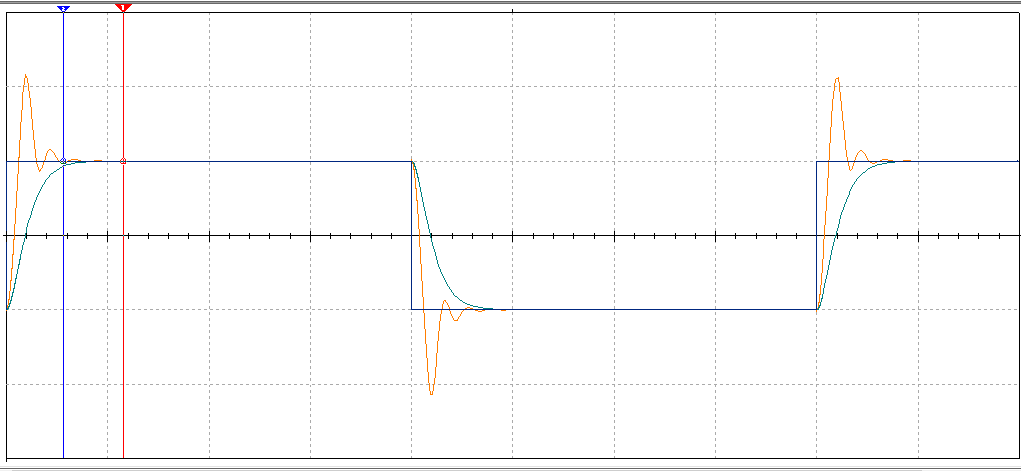
\includegraphics[width=0.5\textwidth]{media1/respuesta-circuito-sobre}
		\caption{Respuesta del sistema control PID frente a la señal cuadrada}
		\label{fig:respuesta-circuito-sobre}
	\end{figure}
	
	Finalmente en las figuras \ref{fig:salida-subamor} y \ref{fig:salida-sobreamor} se pueden apreciar la reducción en el sobreimpulso y el tiempo de establecimiento para cada sistema, verificando de esta forma la eficacia del control PID para modificar el comportamiento de un sistema mediante el ajuste y/o sintonización de constantes.
	
	\begin{figure}[h]
		\centering
		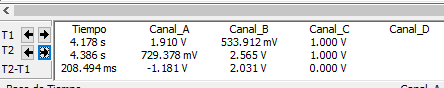
\includegraphics[width=0.5\textwidth]{media1/salida-subamor}
		\caption{Reducción del sobreimpulso para el sistema subamortiguado}
		\label{fig:salida-subamor}
	\end{figure}
	
	\begin{figure}[h]
		\centering
		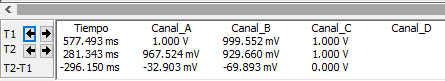
\includegraphics[width=0.5\textwidth]{media1/salida-sobreamor}
		\caption{Reducción del tiempo de respuesta para el sistema sobreamortiguado}
		\label{fig:salida-sobreamor}
	\end{figure}
	\bibliographystyle{IEEEtran}
	\bibliography{biblio}
\end{document}